\newpage
\subsection{Rule based Converging}\label{s:testRuleConverging}

\paragraph{Scenario:} Two \emph{UAS} are approaching an \emph{airway intersection} at \emph{same time} in \emph{controlled airspace} (over 500 feet Above the Ground Level). The mutual position of \emph{UAS} can be classified as \emph{Side approach}. Following \emph{collision hazards} are present:

\begin{enumerate}
    \item \emph{Active Converging Collision Hazard} -  There is an \emph{UAS} approaching from the \emph{right side}, which give him \emph{Right of the Way} and invokes need to actively avoid \emph{Intruder}.

	\item \emph{Passive Converging Collision Hazard} - There is an \emph{UAS} approaching from the \emph{left side}, which gave us \emph{Right of the Way} and imposes an obligation of \emph{active avoidance} on other \emph{UAS}.
	
\end{enumerate}


\noindent\emph{Collision Hazards} must be addressed by \emph{UTM} service in the following manner:


\begin{enumerate}
	\item \emph{Each UAS} in particular \emph{Controlled Space} periodically sends synchronized \emph{Position Notification} messages (tab. \ref{tab:positionNotification}). 
	
	\item \emph{UTM} service receives \emph{Position Notifications} and manages \emph{Collision Case} (tab. \ref{tab:collisionCase}) in \emph{Controlled Space}. 
	
	\item \emph{UTM} detects \emph{Converging Collision Case} with \emph{Collision Point} in  vicinity.
	
	\item \emph{UTM} service Sends \emph{Mandate} to UAS without \emph{Right of the Way} and implements \emph{Normative Directive} on all \emph{UAS} in area.
\end{enumerate}


\noindent\emph{Mission parameters} for both UAS systems are defined in (tab. \ref{tab:missionSetupRuleBasedConvergingScenario}).

\begin{table}[H]
    \centering
    \begin{tabular}{c||c|c||c}
        \multirow{2}{*}{UAS} &\multicolumn{2}{c||}{Position} & \multirow{2}{*}{$\mathscr{WP}_1$} \\\cline{2-3}
          & $[x,y,z]$           & $[\theta,\varpi,\psi]$           & \\\hline\hline
        1 & $[0,20,0]^T $       & $[0^\circ,0^\circ,0^\circ]^T$    & $[40,20,0]^T$\\\hline 
        2 & $[20,0,0]^T $       & $[0^\circ,0^\circ,90^\circ]^T$    & $[20,40,0]^T$\\
    \end{tabular}
    \caption{Mission setup for \emph{Rule based converging} scenario.}
    \label{tab:missionSetupRuleBasedConvergingScenario}
\end{table}


\paragraph{Assumptions:} Following assumptions are valid for this test:

\begin{enumerate}
	\item \emph{Controlled Airspace Airworthiness} - UAS system is equipped with necessary controlled airspace equipment like ADS-B In/Out, Radar, Transponder, etc. Moreover airworthy \emph{UAS} has capability to precisely follow \emph{UTM directives} (max. 5 $\%$ deviation).
	
	\item \emph{C2 (Command \& control) Link Established} - necessary for (UAS $\leftrightarrow$ UAS) and (UAS $\leftrightarrow$ UTM) communication. If \emph{C2} link is lost the \emph{UAS} will enter into \emph{Emergency avoidance mode}.
	
	\item \emph{Decision frame synchronization with UTM} - necessary in discrete C2 environment otherwise \emph{safety margins} needs to be \emph{bloated}.
	
	\item \emph{Both UAS have identical cruising speed} - simplification impacting \emph{UTM} service implementation. \emph{Obstacle Avoidance Framework} can comprehend various intruders speed, with proper \emph{UAS} directives.
\end{enumerate}

\paragraph{Main Goal:} Show possibility of \emph{Converging situation resolution} with \emph{forced safety margin} by \emph{UAS Traffic Management} system.  The \emph{Obstacle Avoidance Framework based on Reach Sets} is used as \emph{Navigation Module}.

\paragraph{Acceptance  Criteria:} Following criteria must be met:

\begin{enumerate}
	\item \emph{Well Clear Condition valid for both UAS} - Both \emph{UAS} must have \emph{minimal required distance} from \emph{other UAS} for all \emph{Converging Maneuver} enforcement time.
	
	\item \emph{Fulfillment of UTM Directives} - Both UAS must stay in \emph{Navigation mode} for all \emph{Converging Maneuver} enforcement time. \emph{UAS without Right Of the Way} must stay away for necessary time, before returning to \emph{Original Navigation waypoint $\mathscr{WP}_1$} following.
\end{enumerate}


\paragraph{Testing Setup:} The \emph{standard test setup} for each UAS defined in (tab. \ref{tab:testMovementOrientations}, \ref{tab:testUASBasicParameters}, \ref{tab:testNavigationGridBasic}, \ref{tab:testAvoidanceGridBasic}, \ref{tab:testUASColoring}) is used with following parameter override:
\begin{enumerate}
	\item \emph{Navigation grid - type} - \emph{ACAS-like} with enabled \emph{Horizontal maneuvers}
\end{enumerate}

This \emph{configuration} is based on assumption that every UAS is in \emph{controlled airspace} in \emph{FL450} (flight level 45000 feet Above Sea Level), without permission for \emph{climb or descent maneuver}. \emph{Rule engine} is initialized in standard \emph{Rules of the air} configuration (fig. \ref{fig:RuleEngineInstanceLevels}).

There is \emph{UTM} service for given \emph{airspace cluster} calculating \emph{collision cases} (tab. \ref{tab:collisionCase}) based on incoming \emph{UAS position notifications} (tab. \ref{tab:positionNotification}).

\paragraph{Simulation Run:} Notable moments from \emph{simulation run} (fig. \ref{fig:testCaseRuleBasedConverging}) are following:

\begin{enumerate}
    \item \emph{Collision Case creation} (fig. \ref{fig:ruleBasedConvergingCollisionCaseCreation}) following events happens in this step:
    \begin{enumerate}[a.]
        \item Two \emph{UAS} are approaching  \emph{airway intersection}: UAS 1 (blue) from left and UAS 2 (cyan) from bottom.
        
        \item They are going to \emph{collide} at point $\mathscr{C}=[20,20,0]^T$ of \emph{Flight Level} (elevation is 45, 000 feet Above Mean Seal Level).
        
        \item UTM service notices future \emph{Collision Situation} and creates \emph{Collision Case}.
        
        \item \emph{Converging Directive} for 8 m from \emph{Collision point} is issued for UAS 1 (blue), because UAS 2 (cyan) has \emph{Right Of the Way}.
        
        \item \emph{Keep Velocity/Heading Directive} is issued for UAS 2 (cyan) to ensure avoidance maneuver success.
        
        \item UAS 1 (blue) corrects its heading according to \emph{UTM} directive.
        
        \item UAS 2 (cyan) stays on claimed course and if its necessary adjust its speed.
        
    \end{enumerate}
    
    \item \emph{Well clear before} (fig. \ref{fig:ruleBasedConvergingWellClearBefore}) UAS 1 (blue) checks the \emph{Collision Point} distance and keeps safe distance given by safety margin. UAS 2 (cyan) checks if there is no intruder in \emph{Avoidance Grid} and if not, stays in \emph{Navigation Mode}.
    
    \item \emph{Well clear after} (fig. \ref{fig:ruleBasedConvergingWellClearAfter}) UAS 2 (cyan) is \emph{after Collision Point}, it can start negotiations of new speed and heading with UTM. UAS 1 (blue) is still enforced to follow \emph{Converging Maneuver} directive, until the outer boundary of \emph{Collision Zone} is reached.
    
    \item \emph{Waypoints reach} (fig. \ref{fig:ruleBasedConvergingWaypointsReach})  UAS 1 (blue) leaves outer boundary of \emph{Collision zone}. Leaving \emph{Converging Maneuver Directive}. UTM closes \emph{Collision Case}.
\end{enumerate}


\begin{figure}[H]
    \centering
    \begin{subfigure}{0.48\textwidth}
    	\centering
        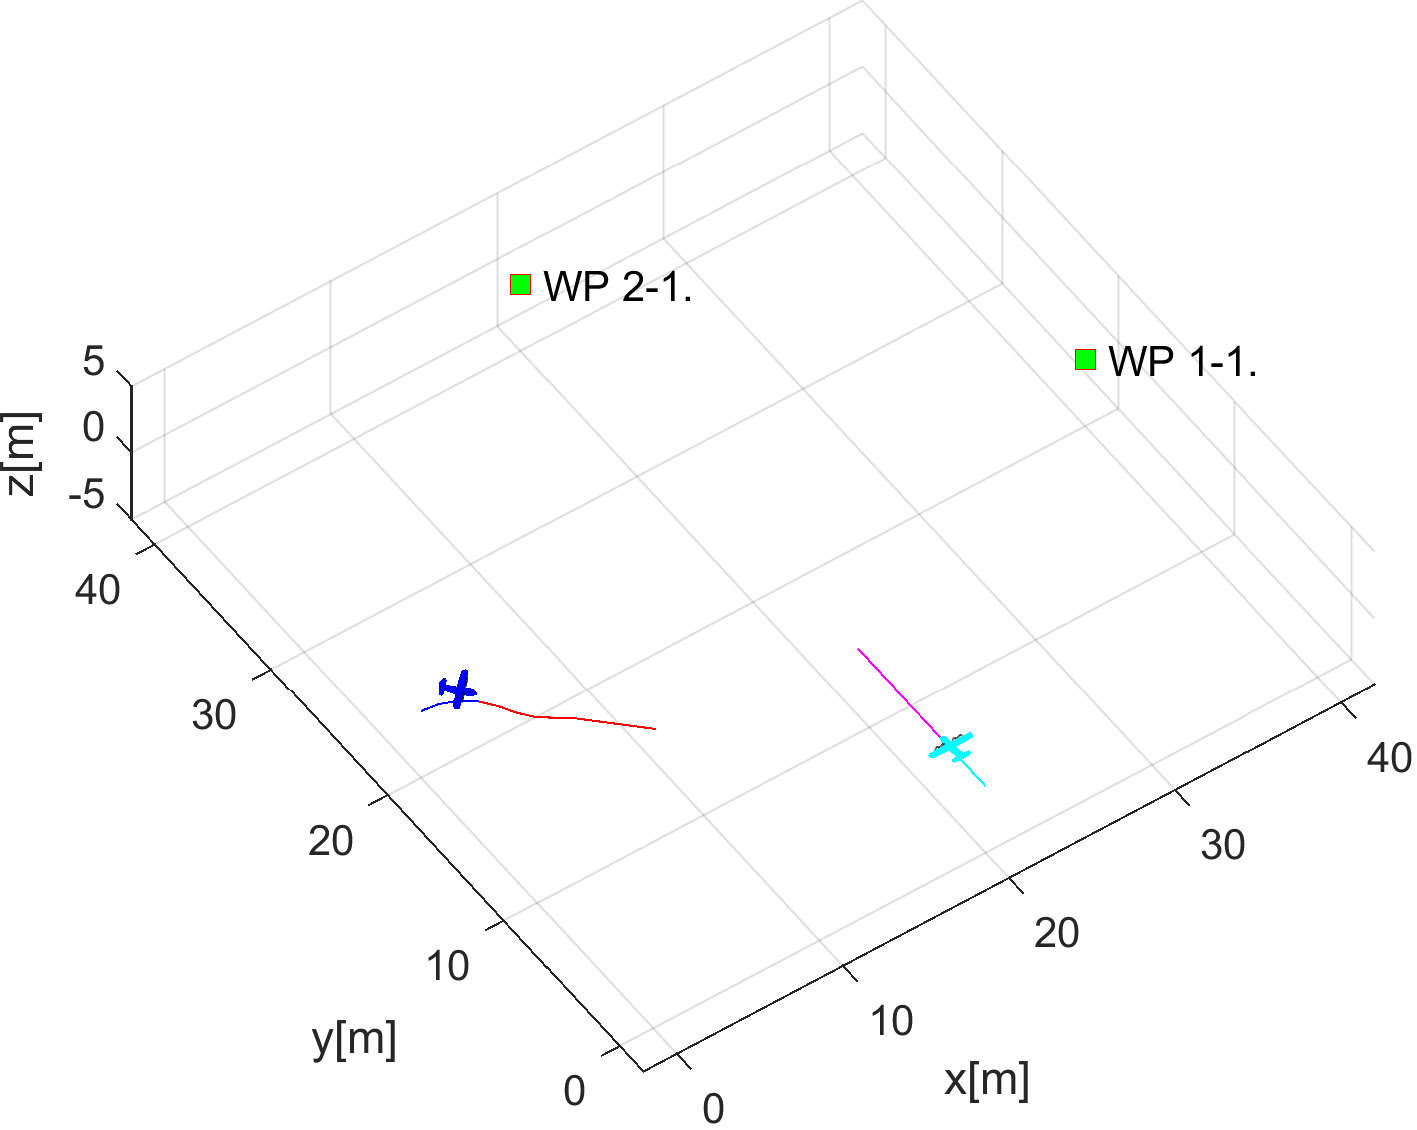
\includegraphics[width=0.9\linewidth]{\FIGDIR/NS048UtmCooperativeConverging00003}
        \caption{Collision case creation.}
        \label{fig:ruleBasedConvergingCollisionCaseCreation}
    \end{subfigure}
    \begin{subfigure}{0.48\textwidth}
    	\centering
        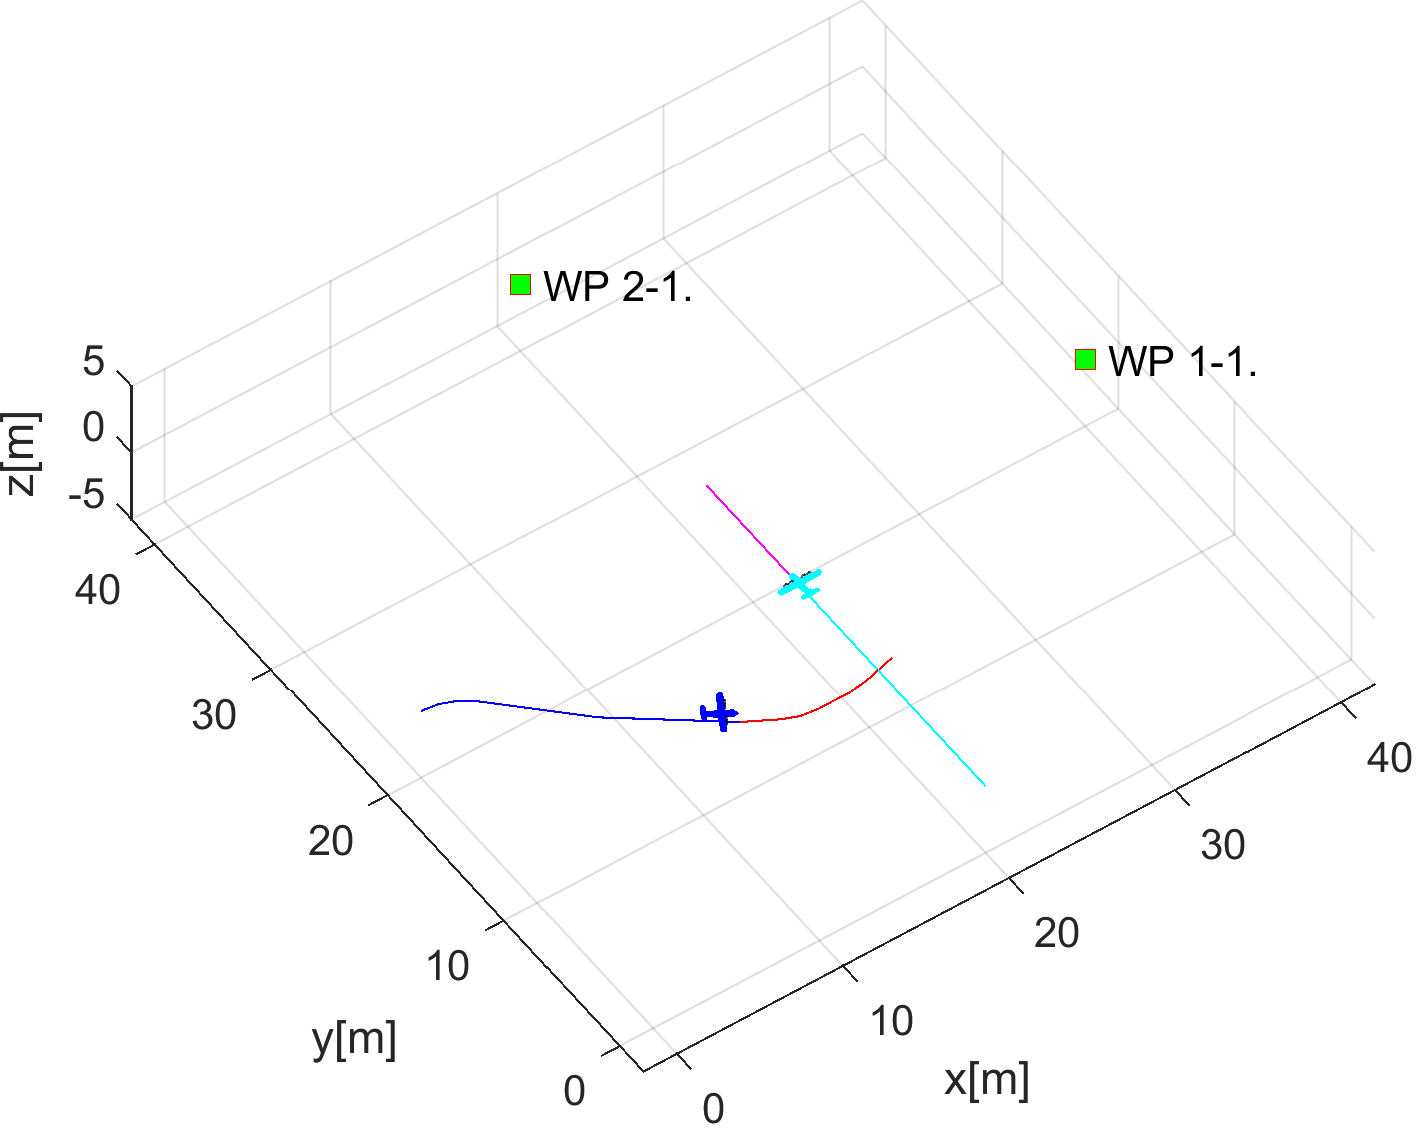
\includegraphics[width=0.9\linewidth]{\FIGDIR/NS049UtmCooperativeConverging00016} 
        \caption{Well clear before.}
        \label{fig:ruleBasedConvergingWellClearBefore}
    \end{subfigure}
    \\
    \begin{subfigure}{0.48\textwidth}
    	\centering
        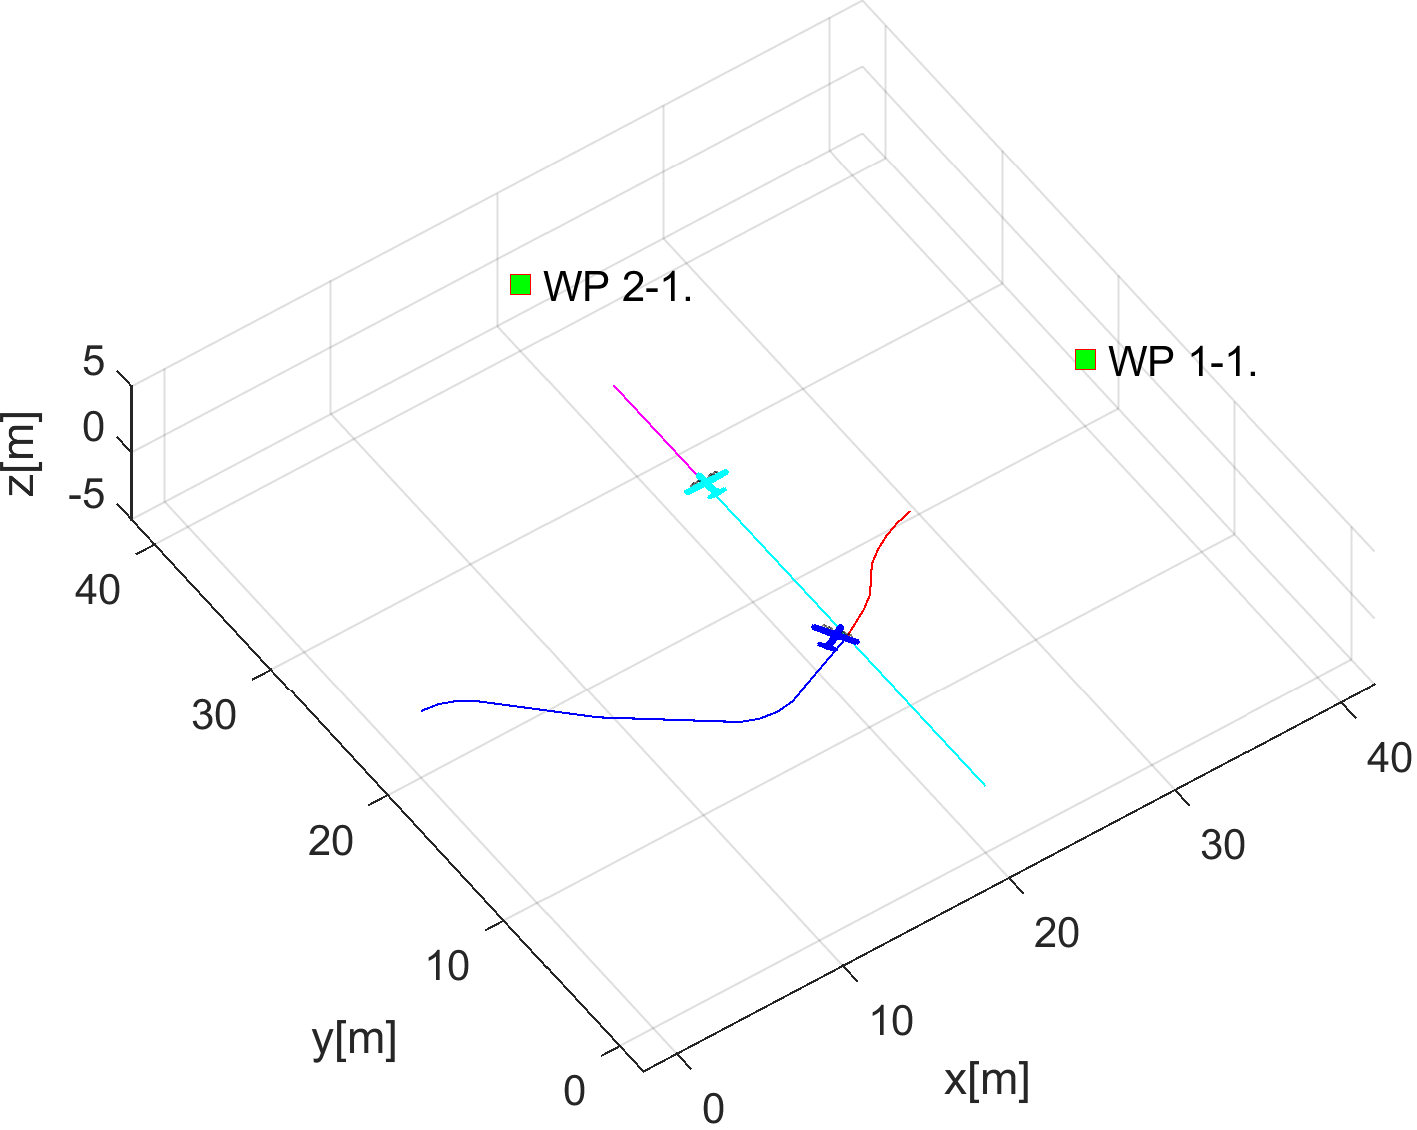
\includegraphics[width=0.9\linewidth]{\FIGDIR/NS050UtmCooperativeConverging00024} 
        \caption{Well clear after.}
        \label{fig:ruleBasedConvergingWellClearAfter}
    \end{subfigure}
    \begin{subfigure}{0.48\textwidth}
    	\centering
        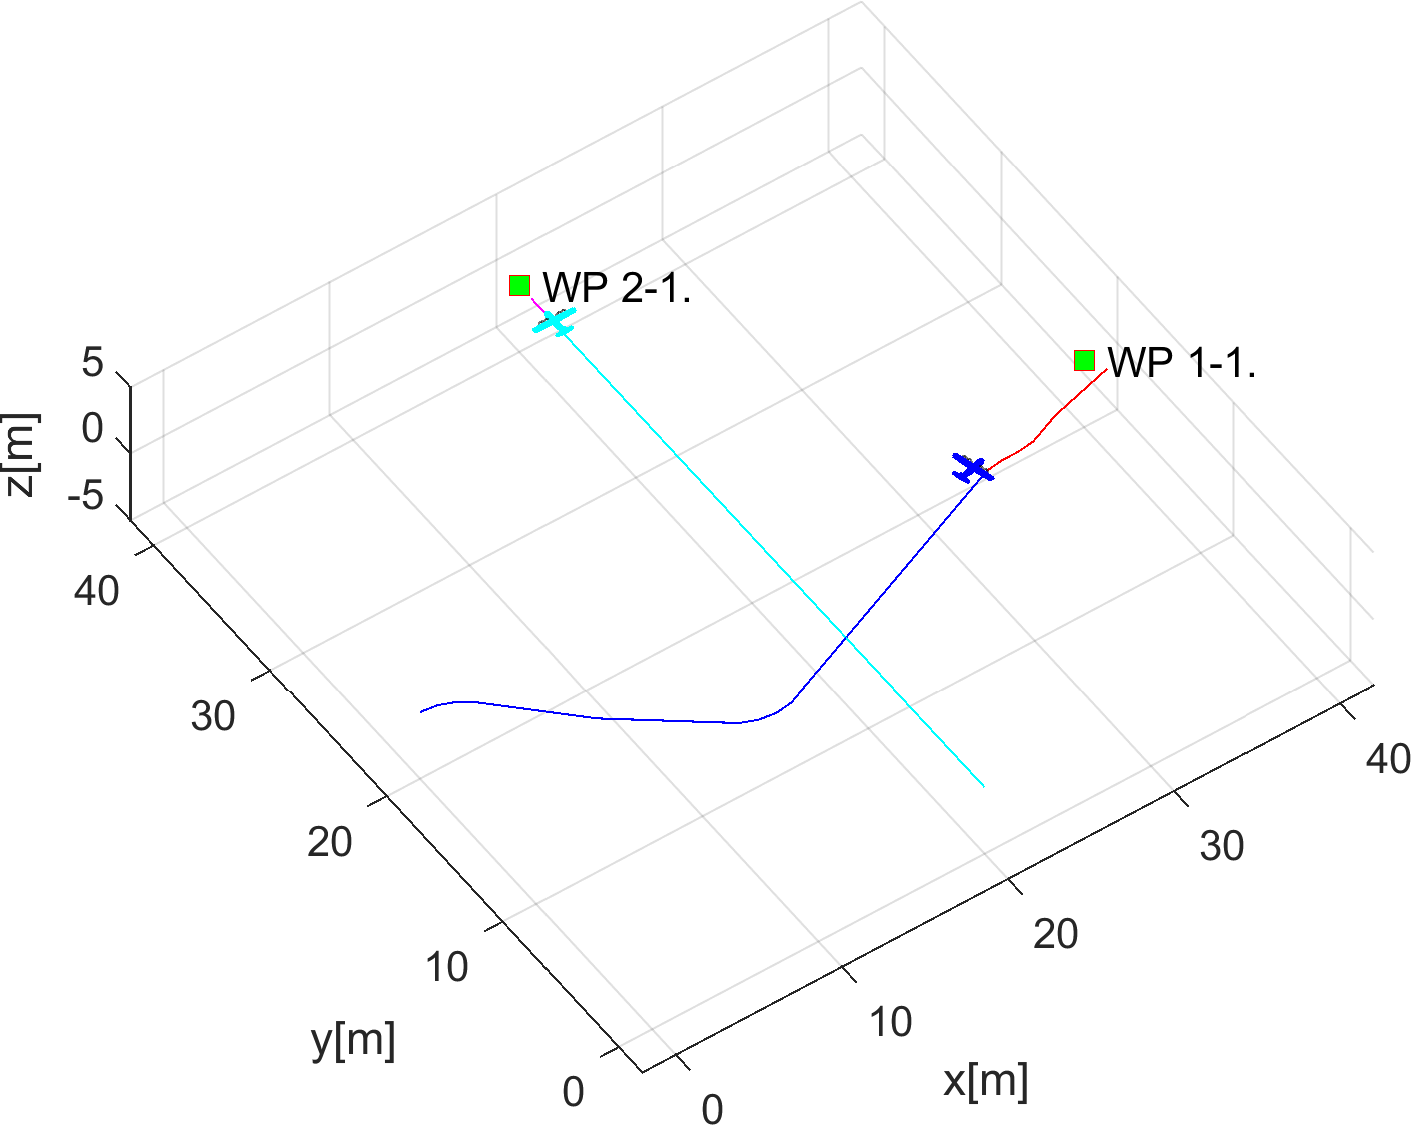
\includegraphics[width=0.9\linewidth]{\FIGDIR/NS051UtmCooperativeConverging00037} 
        \caption{Waypoints reach.}
        \label{fig:ruleBasedConvergingWaypointsReach}
    \end{subfigure}
    \caption{Test scenario for \emph{Rule based converging}. }
    \label{fig:testCaseRuleBasedConverging}
\end{figure}


\paragraph{Collision Case Calculation:} For test scenario in (fig. \ref{fig:testCaseRuleBasedConverging}) where UAS 1 (blue) is converging to avoid UAS 2 (cyan) the \emph{Collision Case} (tab. \ref{tab:collisionCasesRuleBasedConverging}) have been calculated. 

The \emph{Collision point} is at $[20,20,0]$ in \emph{Flight Level} $FL450$ coordinate frame.

The \emph{angle of approach} was evaluated as $90^{\circ}$ which indicates \emph{converging maneuver} in range $70^{\circ} \le angle Of Approach < 130^{\circ}$.

The \emph{mutual position} of UAS 1 (blue) and UAS 2(cyan) is giving the roles: \emph{Right Of the Way} for UAS 2 (cyan) and \emph{Converging} for UAS 1 (blue).

The \emph{safety margin} for \emph{Well Clear} was determined as $3m$ for UAS 1 and $5 m$ for UAS 2. (Note: Well Clear Margin is usually much greater than Near Miss margin). The \emph{Combined Case} margin which was enforced was $8 m$. The mutual distance can not go below this threshold. 


\begin{table}[H]
    \centering
    \begin{tabular}{c|c|c|c|c|c||c|c}
        \multicolumn{6}{c||}{Collision Case}& \multicolumn{2}{c}{Margins} \\ \hline
        id  & UAS & role & \begin{tabular}[c]{@{}c@{}}collision\\ point\end{tabular} & \begin{tabular}[c]{@{}c@{}}angle of\\ approach\end{tabular} & type&  safety  & case  \\ \hline\hline
        % Case 1-2
        \multirow{2}{*}{1-2} & 1   & Converging & \multirow{2}{*}{$[20,20,0]^T$} & \multirow{2}{*}{$90^\circ$} & \multirow{2}{*}{Converging} & 3 & \multirow{2}{*}{8} \\ \cline{2-3} \cline{7-7} & 2   & Right o. W. & & & & 5 & 
    \end{tabular}
    \caption{Collision case for \emph{Rule-based converging} scenario.}
    \label{tab:collisionCasesRuleBasedConverging}
\end{table}


\paragraph{Distance to Safety Margin Evolution:} The safety margin values (well clear) (fig. \ref{fig:testCaseRuleBasedConvergingAvoidancePerformance}) in controlled airspace are much greater than in non-controlled airspace (near miss) (fig. \ref{fig:testCaseEmergencyConvergingAvoidancePerformance}) 

The enforced rule was (rule \ref{tab:ruleConvergingManuever}) with parameters: Collision Point $[20,20,0]^T$ and \emph{Safety Margin} $8$ $m$ as given by Collision Case (tab. \ref{tab:collisionCasesRuleBasedConverging}).

The mutual \emph{UAS distance} (blue line) does not go over \emph{Safety Margin} (red line), which means UAS 1 well clear margin of $3$ $m$ and UAS 2 well clear margin of $5$ $m$ are not broken (fig. \ref{fig:testCaseRuleBasedConvergingAvoidancePerformance}).

\begin{figure}[H]
    \centering
    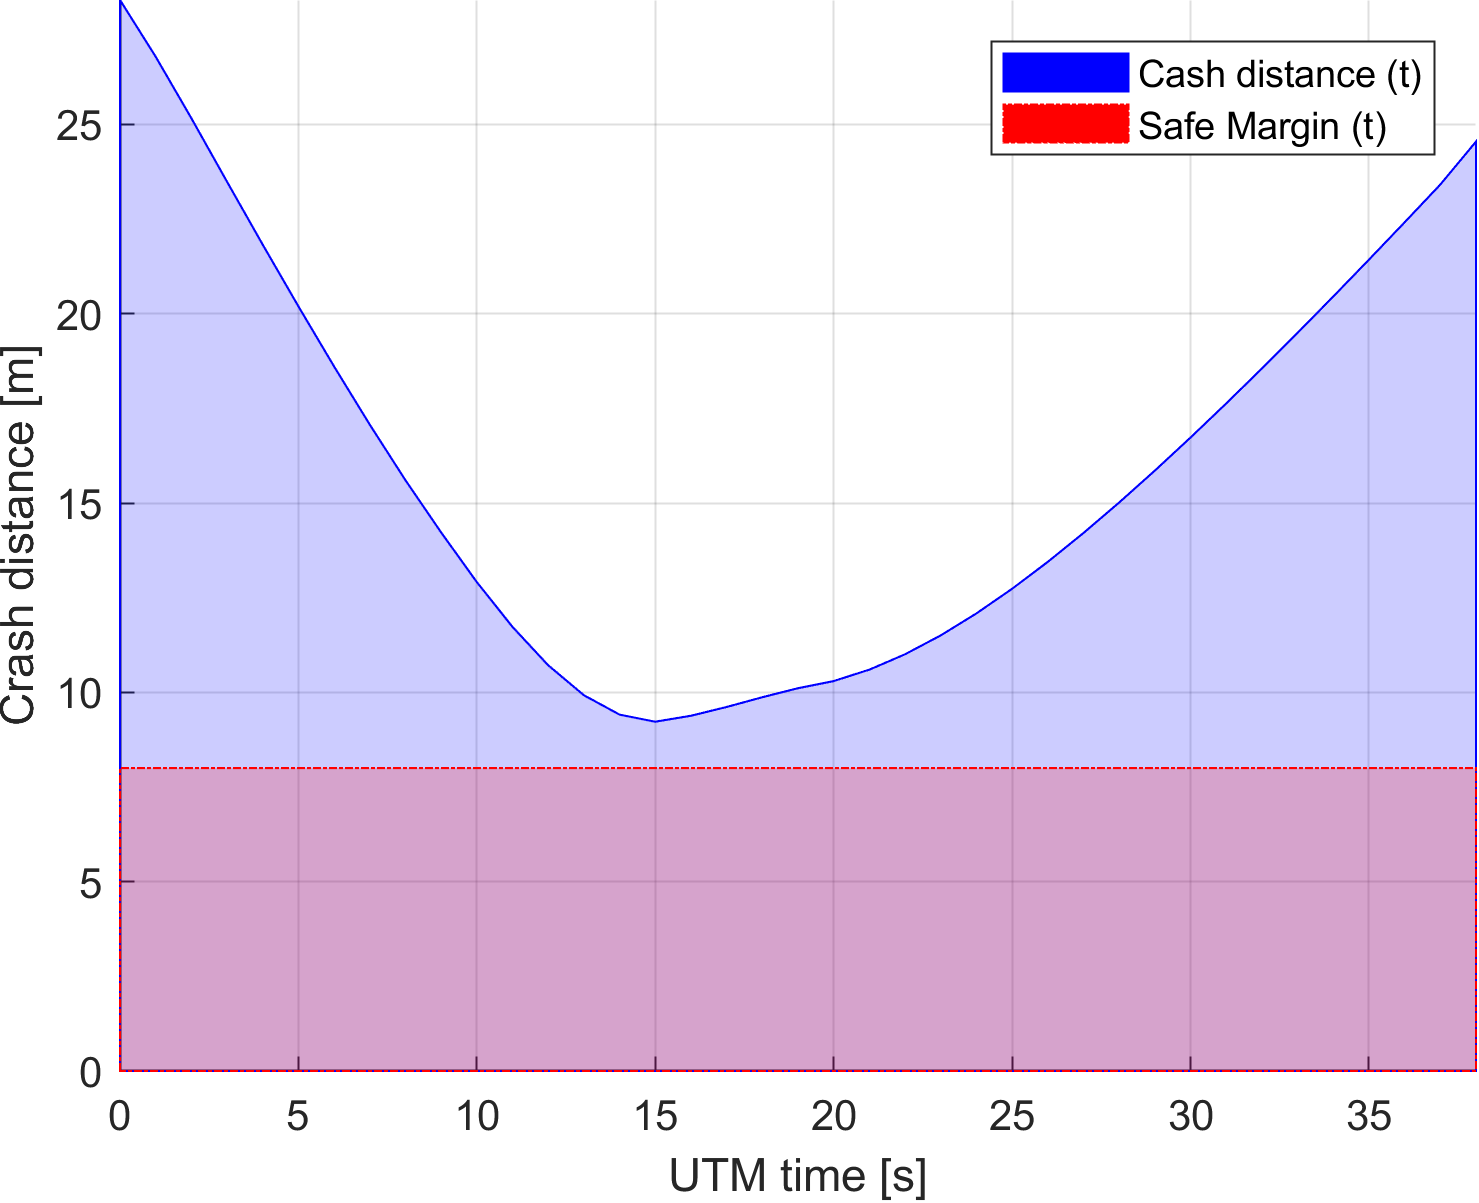
\includegraphics[width=0.55\linewidth]{\FIGDIR/NS052UtmCooperativeConvergingPerformance} 
    \caption{Distance to safety margin evolution for \emph{rule based converging scenario}.}
    \label{fig:testCaseRuleBasedConvergingAvoidancePerformance}
\end{figure}


\paragraph{Distance to Safety Margin Peaks:} \emph{Distance to safety margin peaks} (tab. \ref{tab:testCaseRuleBasedConvergingSafetyMarginDistances}) represent the proximity on UAS mutual distance to \emph{breach of well clear condition} (safety margin). The \emph{breach of well clear condition} was not achieved. The \emph{minimal distance to safety margin} was $1.2240$ $m$. The \emph{maximal distance to safety margin} was $20.2843$ $m$ which represents distance in time of \emph{Collision Case Creation}.

\begin{table}[H]
    \centering
    \begin{tabular}{c||c|c|c}
        \multirow{2}{*}{UAS:} & \multicolumn{3}{c}{Distance to Safety Margin} \\ \cline{2-4} 
                  & min          & max         & breach         \\ \hline\hline
            1-2   & 1.2240       & 20.2843     & false          \\ 
    \end{tabular}
    \caption{Distance to safety margin peaks for \emph{Rule based converging scenario}.}
    \label{tab:testCaseRuleBasedConvergingSafetyMarginDistances}
\end{table}

\newpage
\paragraph{Path Tracking Performance:} \emph{Path tracking} is displayed in (fig. \ref{fig:ruleBasedConvergingTrajectoryTrackingPerformance}). The \emph{UAS} trajectory is divined into \emph{X, Y, Z axis tracking over UTM Time}. The \emph{Reference Trajectory} (green dashed line) interconnect starting position of UAS (green square marked S) an goal waypoint (green square marked 1). The \emph{Executed Trajectory} (blue solid line) reflects real UAS trajectory. 

\begin{enumerate}
    \item UAS 1. (fig, \ref{fig:ruleBasedConvergingUAS1PathTracking}) do steady right side \emph{converging maneuver} (y-axis).
    
    \item UAS 2. (fig. \ref{fig:ruleBasedCovnergingUAS2PathTracking}) follows the reference trajectory precisely, because it has \emph{Right Of the Way}.
\end{enumerate}

\begin{figure}[H]
    \centering
    \begin{subfigure}{0.48\textwidth}
    	\centering
        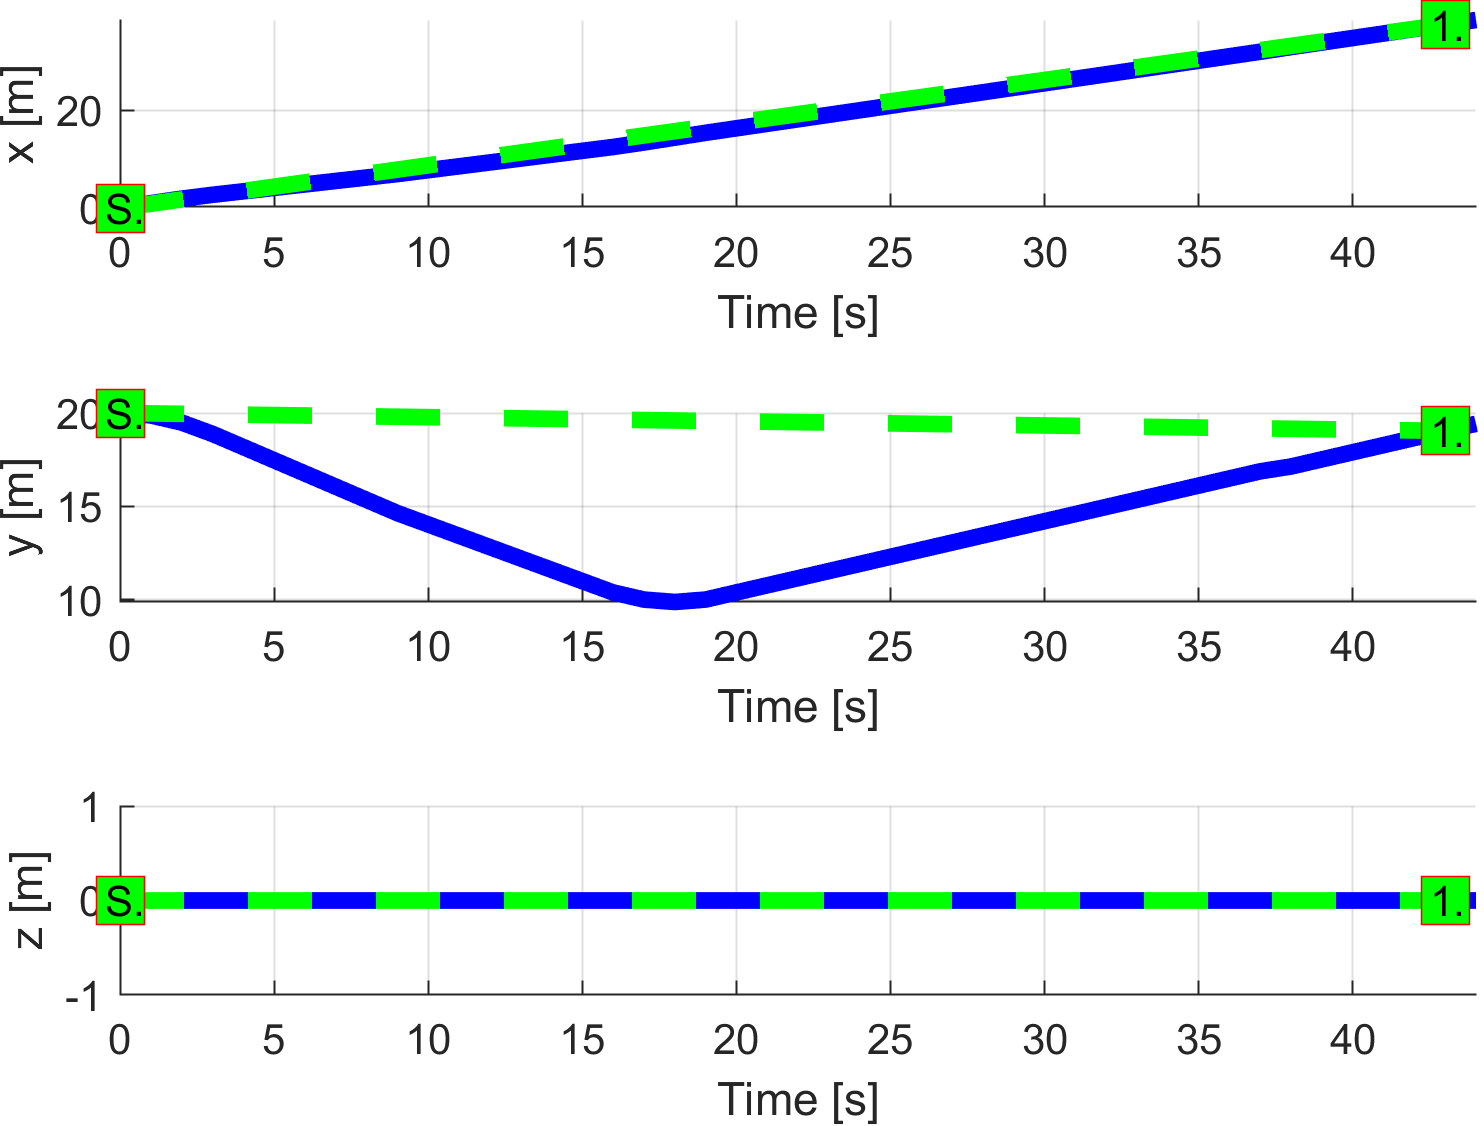
\includegraphics[width=0.9\linewidth]{\FIGDIR/NS053UtmCooperativeConvergingUAV1PathFollowing}
        \caption{UAS 1.}
        \label{fig:ruleBasedConvergingUAS1PathTracking}
    \end{subfigure}
    \begin{subfigure}{0.48\textwidth}
    	\centering
        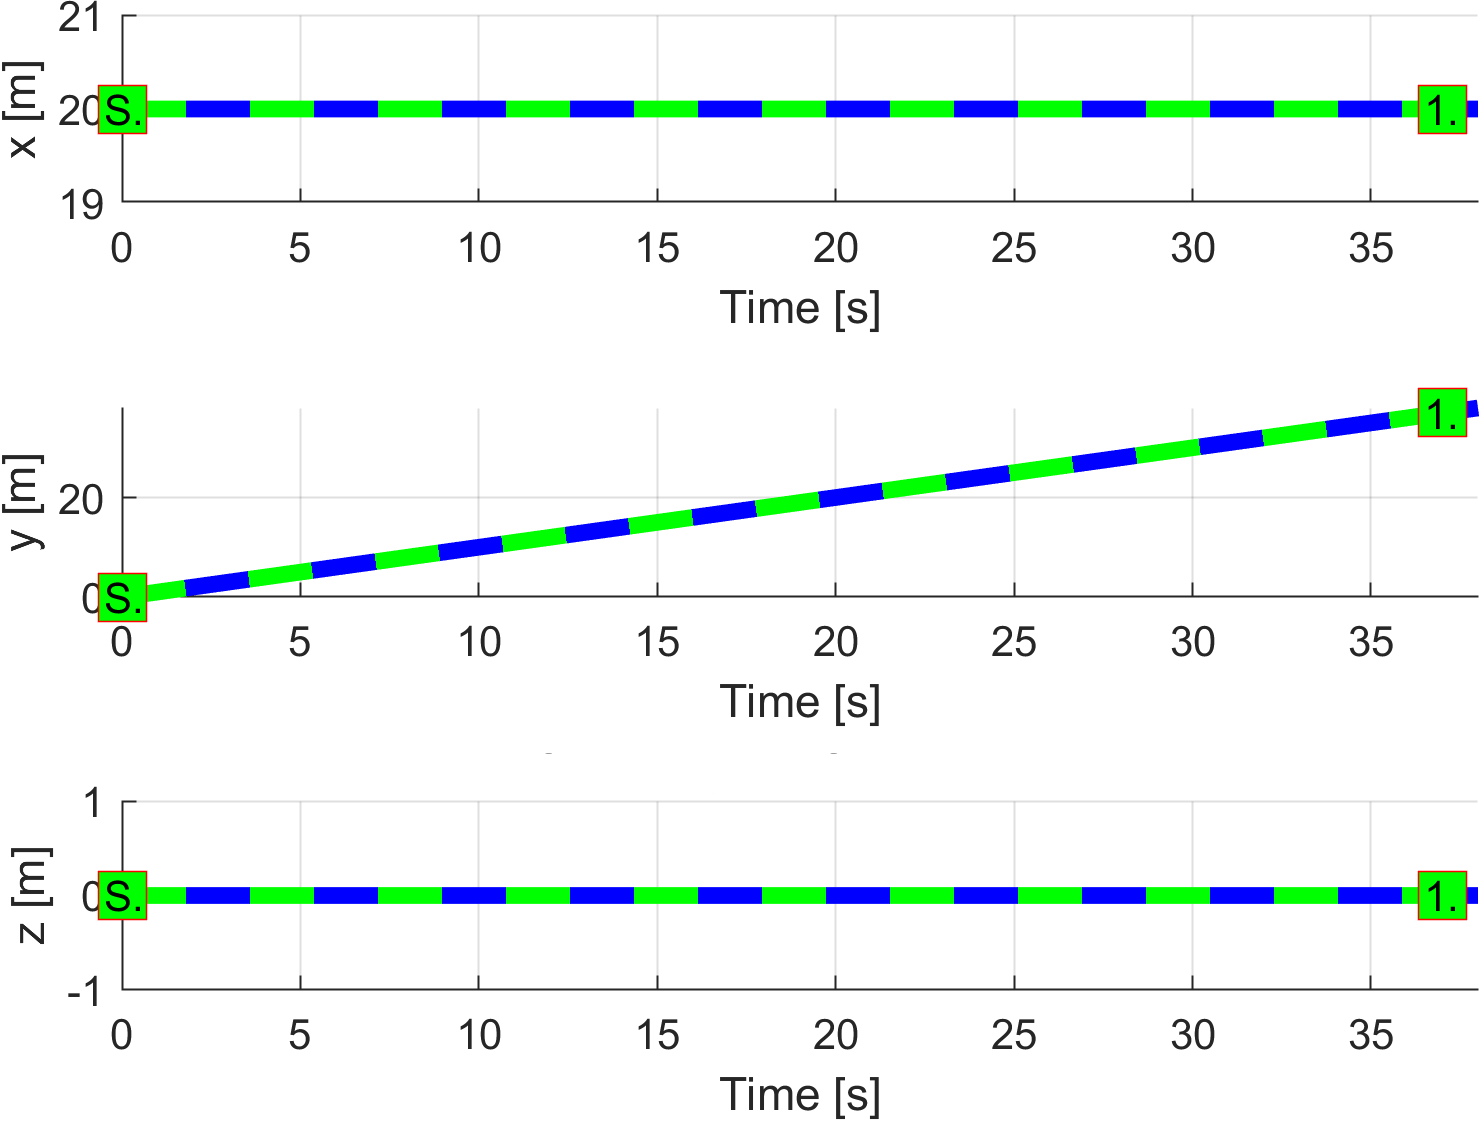
\includegraphics[width=0.9\linewidth]{\FIGDIR/NS054UtmCooperativeConvergingUAV2PathFollowing} 
        \caption{UAS 2.}
        \label{fig:ruleBasedCovnergingUAS2PathTracking}
    \end{subfigure}
    \caption{\emph{Trajectory tracking} for \emph{Rule based converging} test case. }
    \label{fig:ruleBasedConvergingTrajectoryTrackingPerformance}
\end{figure}

\paragraph{Path Tracking Deviations:} Deviations (tab. \ref{tab:pathTrackingParametersForRuleBasedConverging}) are in \emph{expected ranges}, considering the \emph{mission plans} (tab. \ref{tab:missionSetupRuleBasedConvergingScenario}) and \emph{Collision Case} safety margin of $8 m$.

The minimal deviation distance was expected at value of \emph{safety margin} ($8 m$). The maximal deviation was $10.22m$ which is acceptable due the space discretization, UAS dynamic, and, \emph{dynamic decision time}.

\begin{table}[H]
    \centering
    \begin{tabular}{c||c|c}
        \multirow{2}{*}{Param.} & UAS 1     & UAS 2              \\\cline{2-3}
                        & $\mathscr{WP}_1$  & $\mathscr{WP}_1$   \\\hline\hline
          $\max |x|$    & 0                 & 0                  \\\hline
          $\max |y|$    & 10.22             & 0                  \\\hline
          $\max |z|$    & 0                 & 0                  \\\hline
          $\max dist.$  & 10.22             & 0                  \\
    \end{tabular}
    \caption{Path tracking properties for \emph{Rule based converging} scenario.}
    \label{tab:pathTrackingParametersForRuleBasedConverging}
\end{table}

\newpage
\paragraph{Computation Load:} The \emph{computation load} for \emph{scenario} (fig.\ref{fig:ruleBasedCConvergingComputationTime}) shows used time (y-axis) over decision frame (x-axis).

The \emph{computation time} is slightly increased for avoiding UAS 1 during avoidance. The initial increase of computation time UAS 2 is caused by UTM communication demand.

\begin{figure}[H]
    \centering
    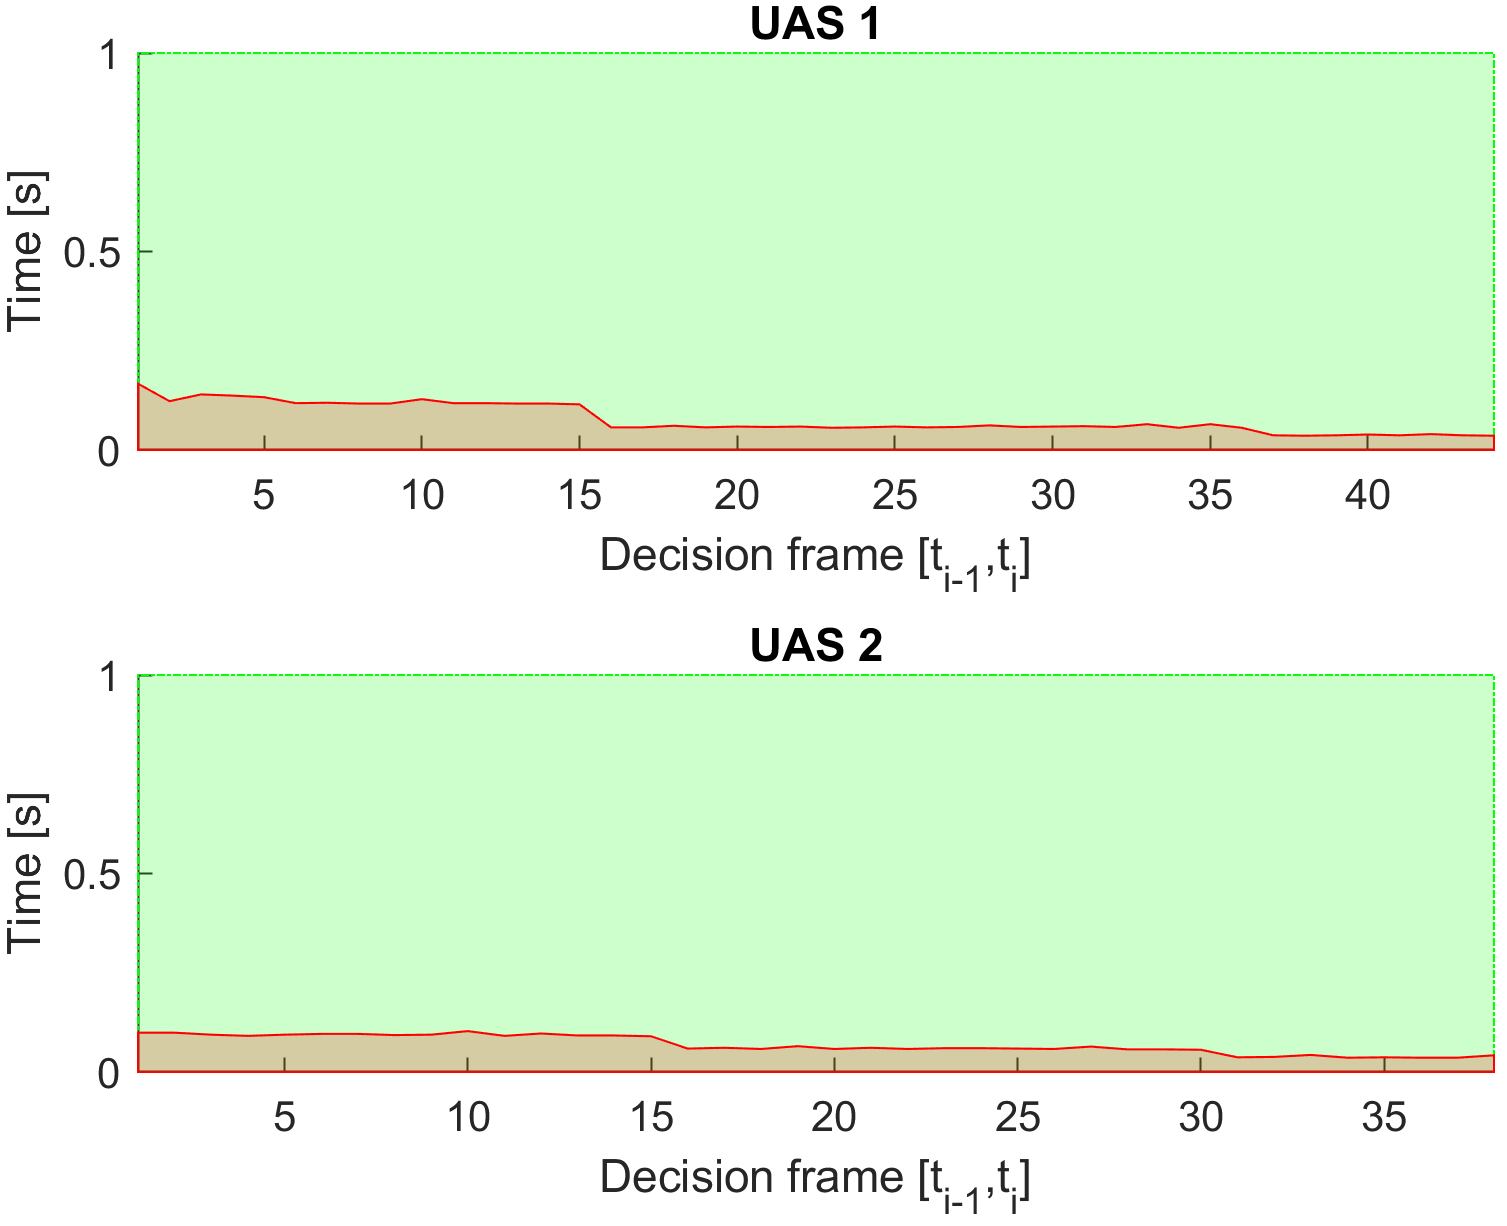
\includegraphics[width=0.65\linewidth]{\FIGDIR/NS099RuleBasedCConvergingComputationTime} 
    \caption{Computation time for \emph{Rule-based converging} scenario.}
    \label{fig:ruleBasedCConvergingComputationTime}
\end{figure}